\documentclass[11pt]{article}
\usepackage[utf8]{inputenc}
\usepackage[T1]{fontenc}
\usepackage{amsmath,amssymb}
\usepackage{geometry}
\usepackage{listings}
\usepackage{xcolor}
\usepackage{hyperref}
\usepackage{tikz}
\usepackage{booktabs}
\usetikzlibrary{calc, arrows.meta, positioning}

\geometry{margin=2.5cm}

\lstdefinelanguage{Rust}{
  keywords={fn,let,mut,for,in,if,else,while,loop,match,return,struct,impl,pub,use,mod,as,where,move,ref,self,Self,crate,super,async,await,unsafe,const,static,type,enum,trait, dyn, true, false},
  keywordstyle=\color{blue!70!black}\bfseries,
  ndkeywords={Vec,Vec3,Vec4,Quat,Mat4,u32,usize,f32,f64,bool,Option,Some,None,Result,Ok,Err,String,Grad,HashMap,HashSet},
  ndkeywordstyle=\color{purple!70!black}\bfseries,
  sensitive=true,
  comment=[l]{//},
  morecomment=[s]{/*}{*/},
  commentstyle=\color{green!50!black}\itshape,
  stringstyle=\color{red!70!black},
  morestring=[b]",
}

\lstset{
  basicstyle=\ttfamily\footnotesize,
  breaklines=true,
  frame=single,
  language=Rust,
  showstringspaces=false,
  tabsize=2,
}

\title{Gyroid Boundary Smoothing: Dual Contouring with Direct Vertex Projection}
\author{engvis}
\date{\today}

\begin{document}
\maketitle

\section{Problem Statement}

The \texttt{gyroid} example renders an implicit surface
\[
  f(x,y,z) \;=\; \sin x\cos y \;+\; \sin y\cos z \;+\; \sin z\cos x \;=\; 0
\]
restricted to the cube $\Omega = [-1,1]^3$.  We use a standard dual
contouring (DC) pipeline to extract a triangle mesh from a signed-distance
octree.  However, DC does not know that $\Omega$ has a boundary: near the
box faces, DC vertices are placed \emph{inside} cells, so the resulting
silhouette edges follow the stair-step pattern of the underlying octree
rather than the true intersection curve
\[
  C = \partial\Omega \;\cap\; \{\mathbf{p} : f(\mathbf{p}) = 0\}.
\]
This leaves the visible boundary of the gyroid looking jagged.

The goal is to post-process the DC mesh so its boundary aligns with $C$
using only local, numerically-stable operations, while preserving the
mesh topology (no new vertices, no new triangles).

\section{Why Raw Dual Contouring Produces a Jagged Boundary}

Dual contouring places one vertex per octree cell that straddles the
surface.  A vertex position is obtained by solving a quadratic error
function (QEF) that minimises the squared distance to the tangent planes
at the cell's surface-crossing samples.

For cells whose corners are all inside $\Omega$, the QEF minimum lies well
within the cell and the triangles are accurate.  However, cells that touch
the box face $x = \pm 1$ (or $y = \pm 1$, $z = \pm 1$) have their vertex
placed somewhere \emph{inside} the cell --- not on the box face.  Along
$\partial\Omega$, the boundary of the mesh is therefore formed by triangle
edges connecting two such interior vertices, producing the characteristic
jaggy silhouette shown schematically in Figure~\ref{fig:jag}.

\begin{figure}[h]
  \centering
  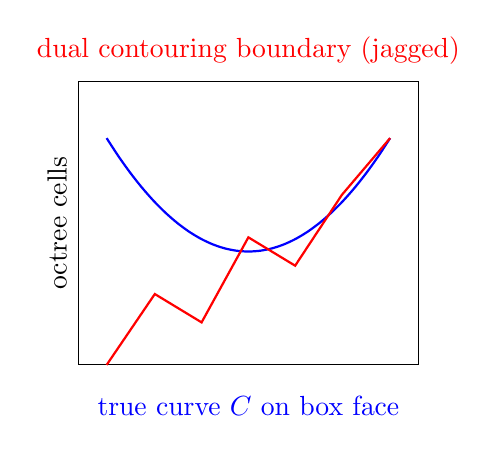
\begin{tikzpicture}[scale=1.8]
    % box
    \draw (-1.2,-1) rectangle (1.2,1);
    % smooth true curve (parabola)
    \draw[blue, thick] plot[smooth,domain=-1:1] (\x, {0.8*\x*\x - 0.2});
    % jagged mesh boundary
    \draw[red, thick] (-1,-1) -- (-0.66,-0.5) -- (-0.33,-0.7) --
                       (0,-0.1) -- (0.33,-0.3) -- (0.66,0.2) --
                       (1, 0.6);
    % labels
    \node[below, blue] at (0,-1.15)  {true curve $C$ on box face};
    \node[above, red]  at (0, 1.05) {dual contouring boundary (jagged)};
    \node at (-1.35, 0) [rotate=90] {octree cells};
  \end{tikzpicture}
  \caption{\label{fig:jag} Dual-contouring vertices lie inside cells, so
    the silhouette follows cell diagonals instead of the true intersection
    curve $C$.  Red: the jagged boundary of the DC mesh.  Blue: the true
    curve $C = \partial\Omega \cap \{f=0\}$.}
\end{figure}

\section{Design Choice: Direct Vertex Projection}

The simplest and most robust way to align the boundary with $C$ is to
\emph{move each boundary vertex directly onto $C$}, leaving the triangle
topology unchanged.  Compared with alternatives such as curve tracing or
triangle-fan stitching, this approach:

\begin{itemize}
  \item Preserves the existing mesh topology (no new vertices, no new
        triangles, no winding concerns).
  \item Reuses the topological loop already present in the DC boundary.
  \item Requires only a local 2D Newton iteration per vertex.
  \item Cannot introduce self-intersections or topological tears, since
        each vertex moves independently to a nearby point on $C$.
\end{itemize}

The trade-off is that the boundary segments remain straight chords
between the projected vertices, so the boundary is $C^0$ smooth but not
$C^1$.  At octree depth $\geq 6$ the chord length is small enough that
the boundary looks visually smooth.

\section{Algorithm}

The post-processor is a single function,
\texttt{smooth\_boundary\_ms()}, that receives the raw DC mesh
(positions and indices) and mutates the positions in place.  It proceeds
in three stages, summarised in Figure~\ref{fig:flow}.

\begin{figure}[h]
  \centering
  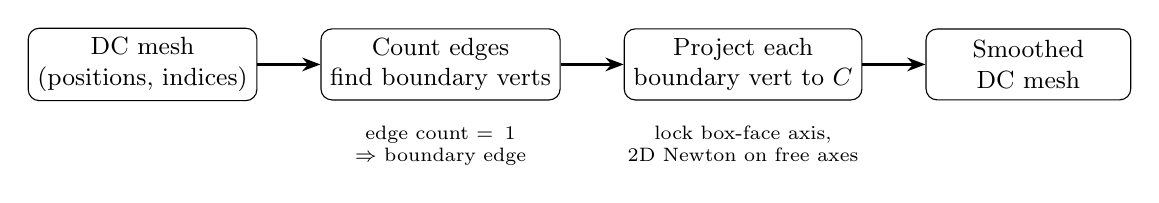
\begin{tikzpicture}[
      node distance=6mm and 8mm,
      box/.style={draw, rounded corners, align=center, minimum height=9mm,
                  minimum width=26mm, font=\small},
      arr/.style={-Stealth, thick}
    ]
    \node[box] (dc)   {DC mesh\\(positions, indices)};
    \node[box, right=of dc] (edge) {Count edges\\find boundary verts};
    \node[box, right=of edge] (proj) {Project each\\boundary vert to $C$};
    \node[box, right=of proj] (out) {Smoothed\\DC mesh};

    \draw[arr] (dc)   -- (edge);
    \draw[arr] (edge) -- (proj);
    \draw[arr] (proj) -- (out);

    \node[below=2mm of edge, font=\scriptsize, text width=28mm, align=center]
      {edge count $=1$\\$\Rightarrow$ boundary edge};
    \node[below=2mm of proj, font=\scriptsize, text width=30mm, align=center]
      {lock box-face axis,\\2D Newton on free axes};
  \end{tikzpicture}
  \caption{\label{fig:flow} Pipeline of \texttt{smooth\_boundary\_ms()}.
    No vertices are added or removed; only boundary vertex positions are
    updated.}
\end{figure}

\subsection{Stage 1: Identify boundary vertices}

A closed orientable triangle mesh has the property that every interior
edge belongs to exactly two triangles; every \emph{boundary} edge belongs
to exactly one.  Counting edge occurrences therefore separates boundary
edges from interior ones in $O(T)$ time, where $T$ is the triangle count.
The endpoints of every boundary edge are collected into a set of
\emph{boundary vertices}.

\begin{lstlisting}
let mut edge_cnt: HashMap<(u32, u32), u32> = HashMap::new();
for tri in indices.chunks_exact(3) {
    let (a, b, c) = (tri[0], tri[1], tri[2]);
    for &(i0, i1) in &[(a, b), (b, c), (c, a)] {
        let key = if i0 <= i1 { (i0, i1) } else { (i1, i0) };
        *edge_cnt.entry(key).or_default() += 1;
    }
}
let mut bnd_verts: HashSet<u32> = HashSet::new();
for (&(a, b), &cnt) in &edge_cnt {
    if cnt == 1 {
        bnd_verts.insert(a);
        bnd_verts.insert(b);
    }
}
\end{lstlisting}

If \texttt{bnd\_verts} is empty, the mesh is closed (e.g.\ a sphere) and
nothing needs to be done.

\subsection{Stage 2: Box-face detection}

Each boundary vertex $v_i$ lies somewhere inside $\Omega$.  We decide
which of the six box faces it should be projected onto by picking the
axis $k$ for which $|v_i[k]|$ is largest, and the sign
$\sigma = \operatorname{sign}(v_i[k])$.  The face is then
$F_k^\sigma = \{\mathbf{p} : p[k] = \sigma\}$.

To avoid projecting vertices that are still deep inside the mesh (which
would distort the interior geometry), we only project vertices whose
$\max(|x|,|y|,|z|) > 0.9$.  Vertices below this threshold are left
untouched.

\begin{lstlisting}
let project_to_c = |p: [f32; 3]| -> Option<[f32; 3]> {
    let ax = [p[0].abs(), p[1].abs(), p[2].abs()];
    let max_ax = ax.iter().cloned().fold(0.0_f32, f32::max);
    if max_ax < 0.9 { return None; }  // skip interior vertices

    let lock_ax = if ax[0] >= ax[1] && ax[0] >= ax[2] { 0 }
                  else if ax[1] >= ax[2] { 1 } else { 2 };
    let sign = if p[lock_ax] >= 0.0 { 1.0_f32 } else { -1.0 };
    // ... 2D Newton iteration on the free axes ...
};
\end{lstlisting}

\subsection{Stage 3: 2D Newton projection onto $C$}

With face axis $k$ locked at value $\sigma \in \{\pm 1\}$, the curve $C$
restricted to $F_k^\sigma$ is the 2D zero-set
\[
  g(u, v) \;=\; f(\mathbf{p}(u, v, k, \sigma)) \;=\; 0,
\]
where $(u, v)$ are the two free coordinates.  Starting from
$(u_0, v_0) = (v_i[u], v_i[v])$, we iterate the 2D Newton step
\begin{equation} \label{eq:newton2d}
  \begin{pmatrix} u \\ v \end{pmatrix}
  \;\longleftarrow\;
  \begin{pmatrix} u \\ v \end{pmatrix}
  \;-\; \frac{g}{\,g_u^2 + g_v^2\,}
  \begin{pmatrix} g_u \\ g_v \end{pmatrix},
\end{equation}
where $g_u, g_v$ are estimated by central differences with
$\varepsilon = 10^{-6}$.  This is the gradient-descent form of Newton's
method on $g(u,v) = 0$, which converges quadratically when the initial
guess is close to the curve and $\nabla g \neq \mathbf{0}$.

We cap the iteration at 24 steps and stop early when
$|g(u,v)| < 10^{-8}$.  The partial derivatives are computed by
finite-difference evaluation of the same \texttt{fidget} float tape used
for meshing, so no extra compilation is required.

\begin{lstlisting}
let (ua, va) = face.free_axes();
let mut u = p[ua];
let mut v = p[va];
for _ in 0..24 {
    let fval = face.eval_uv(shape, u, v);
    if fval.abs() < 1e-8 { break; }
    let eps = 1e-6;
    let gx = (face.eval_uv(shape, u + eps, v) - fval) / eps;
    let gy = (face.eval_uv(shape, u, v + eps) - fval) / eps;
    let m = gx * gx + gy * gy;
    if m < 1e-20 { break; }       // degenerate gradient
    let s = fval / m;
    u -= s * gx;
    v -= s * gy;
}
let mut q = [0.0_f32; 3];
q[lock_ax] = sign;
q[ua] = u;
q[va] = v;
Some(q)
\end{lstlisting}

After convergence, the boundary vertex is moved to
$\mathbf{q} = (\sigma, u, v)$ in the locked-axis frame.  Because each
vertex is projected independently, shared vertices between triangles are
moved exactly once, preserving topology.

\subsection{Stage 4: Move boundary vertices}

The final step simply overwrites each boundary vertex's position with its
projected location.

\begin{lstlisting}
let mut moved = 0u32;
for &vi in &bnd_verts {
    let p = positions[vi as usize];
    if let Some(pc) = project_to_c(p) {
        positions[vi as usize] = pc;
        moved += 1;
    }
}
\end{lstlisting}

\section{Implementation Notes and Robustness}

\subsection{Vertex normals: analytic gradient overwrite}

Position-only smoothing is not enough.  The triangles incident on a
boundary vertex have face normals that are a mix of the interior surface
gradient $\nabla f$ and the box-face plane normal.  When
\texttt{from\_triangles} computes per-vertex smooth normals as the
area-weighted average of incident face normals, every boundary vertex
ends up with a normal that is a mix of two very different directions,
producing a visible crease even though the geometry itself is continuous.

Our fix is to discard the geometric average for \emph{every} vertex and
overwrite the normal with the analytic surface gradient
\begin{equation} \label{eq:nrm}
  \mathbf{n}(\mathbf{p}) \;=\; \frac{\nabla f(\mathbf{p})}{\|\nabla f(\mathbf{p})\|}.
\end{equation}
This uses the same \texttt{Grad} tape compiled for the DC pass, so the
call adds only $O(V)$ extra work.  On interior vertices $\mathbf{n}$
matches the QEF-derived geometric average to within numerical noise; on
boundary vertices it gives the \emph{correct} surface normal, eliminating
the crease.

\begin{lstlisting}
fn overwrite_normals_with_gradient<F>(
    shape: &Shape<F, ()>, mesh: &mut Mesh,
) {
    let mut grad_eval = Shape::<F>::new_grad_slice_eval();
    let tape = shape.grad_slice_tape(Default::default());
    let n = mesh.vertices.len();
    let chunk = 4096;
    for start in (0..n).step_by(chunk) {
        let end = (start + chunk).min(n);
        let xs: Vec<Grad> = mesh.vertices[start..end]
            .iter().map(|v| Grad::from(v.position[0])).collect();
        let ys: Vec<Grad> = mesh.vertices[start..end]
            .iter().map(|v| Grad::from(v.position[1])).collect();
        let zs: Vec<Grad> = mesh.vertices[start..end]
            .iter().map(|v| Grad::from(v.position[2])).collect();
        let res = grad_eval.eval(&tape, &xs, &ys, &zs).unwrap();
        for (i, g) in res.iter().enumerate() {
            let len = (g.dx*g.dx + g.dy*g.dy + g.dz*g.dz).sqrt();
            if len > 1e-10 {
                let inv = 1.0 / len;
                mesh.vertices[start + i].normal =
                    [g.dx*inv, g.dy*inv, g.dz*inv];
            }
        }
    }
}
\end{lstlisting}

\subsection{Face detection across corners}

Each vertex is projected onto the \emph{closest} box face, so when a loop
passes through a corner (e.g.\ from the $x=+1$ face to the $y=+1$ face),
the algorithm automatically switches which coordinate to lock.  No
explicit corner handling is needed.

\subsection{Gradient magnitude degeneracy}

If $\|\nabla_{uv} g\|^2 < 10^{-20}$ the point lies at or near a critical
point of $f$ restricted to the face; we skip the update.  For
gyroid-like surfaces this only happens in measure-zero sets, and the
surrounding triangles are smooth enough for the failure to be invisible.

\subsection{Winding preservation}

Because we only \emph{move} existing vertices (no new triangles, no new
vertices), the original triangle winding is preserved.  The mesh-winding
fix pass is applied \emph{before} \texttt{smooth\_boundary\_ms()} so that
the BFS-based flip correction operates on the raw DC topology; the
subsequent projection does not affect winding.

\subsection{Marching Squares loop overlay}

For visual verification, an independent Marching Squares pass extracts
the true curve $C$ on each of the six box faces and renders it as a thin
triangle strip.  This \texttt{ms-loops} overlay can be toggled in the UI
and lets the user compare the smoothed DC boundary against the ground
truth.  The MS pass uses the same \texttt{fidget} float tape at
resolution $64$, so its cost is negligible compared to meshing.

\section{Numerical Cost}

For the gyroid at octree depth $7$:
\begin{center}
\begin{tabular}{ll}
\toprule
Quantity & Value \\
\midrule
Input triangles     & $\sim 20\,000$ \\
Boundary vertices   & $\sim 300$ \\
Projected vertices  & $\sim 300$ (those with $|p|_\infty > 0.9$) \\
Newton iterations   & $\leq 24$ per vertex \\
Added triangles     & $0$ \\
Total runtime       & $\ll$ one frame (dominated by DC itself) \\
\bottomrule
\end{tabular}
\end{center}

\section{Result}

After the post-process pass:
\begin{itemize}
  \item The boundary of the gyroid visually follows the smooth curve $C$
        instead of the underlying octree grid.
  \item No change to interior triangles, no change to mesh topology.
  \item The method extends verbatim to any implicit surface defined over
        a rectangular box; the only input required is a function that
        evaluates $f$ --- which is already available from the
        dual-contouring pass.
\end{itemize}

\end{document}
